\documentclass[reprint,amsmath,amssymb,aps,showpacs,superscriptaddress,prl]{revtex4-1}

\usepackage{graphicx}
\usepackage{bm}
\usepackage{epsfig}
\usepackage{amssymb}
\usepackage{amsfonts}
\usepackage{braket}
\usepackage{color}
\usepackage{epstopdf}
\epstopdfsetup{update}
\usepackage{hyperref}
\usepackage{float}
\restylefloat{table}
\usepackage{bibentry}
\usepackage{multirow}
\usepackage[caption=false]{subfig}
\newcommand{\ba}{\begin{eqnarray}}
\newcommand{\ea}{\end{eqnarray}}
\newcommand{\bd}{\begin{displaymath}}
\renewcommand{\v}[1]{{\bf #1}}
\newcommand{\nn}{\nonumber \\}

\graphicspath{{figures/}}% Put all figures in this directory.

\begin{document}
%
\title{Machine-learning Skyrmions}

\author{Vinit Kumar Singh}
\email[Electronic address:$~~$]{vinitsingh911@gmail.com}
\affiliation{Department of Physics, Indian Institute of Technology, Kharagpur 721302, India}
\author{Jung Hoon Han}
\email[Electronic address:$~~$]{hanjh@skku.edu}
\affiliation{Department of Physics, Sungkyunkwan University, Suwon 16419, Korea}
\date{\today}

\begin{abstract}
Principles of machine learning (ML) are applied to models that support skyrmion phases in two dimensions. Most successful predictions were found when a convolutional neural network (CNN) layer was inserted as well as several layers of neural networks. A new training scheme based on features of the input configuration such as magnetization and spin chirality is introduced to make reliable predictions on the mixed phases, consisting of either a mixture of spiral and skyrmions or of skyrmions and ferromagnets. It proved possible to further train external parameters such as the external magnetic field and temperature and make reliable predictions on them. The predictive capacity of the ML continued to apply to configurations that are not generated by the original Hamiltonian used in the training stage, but a different Hamiltonian adiabatically connected to the original one.
\end{abstract}
%\pacs{75.78.-n, 75.10.Hk, 75.70.Kw, 75.78.Cd}
\maketitle

The basic strategy behind teaching ML algorithm to recognize various phases of many-body systems~\cite{melko16,wang16,melko17,melko17b,melko17c,tanaka17,scalettar17,wetzel17,wetzel17b,iso18,kim18,zhai17,scalettar17,beach18,zhai18,russian18}, whether classical or quantum, is to train it on many examples of many-body configurations together with answers to the phases to which they belong.  After the successful implementation of supervised learning as such, the ML algorithm can predict the phase of a new configuration, not drawn from the previous training set. Most studies in recent years have focused on the transition between ordered and disordered phases separated with a second-order critical point. Following the natural progression in the level of sophistication, models studied with the ML method have evolved from Ising\cite{melko16,wang16,melko17,melko17b,melko17c,tanaka17,scalettar17,wetzel17,wetzel17b,iso18,kim18} to planar (XY)\cite{zhai17,scalettar17,wetzel17b,beach18,zhai18}, and most recently to Heisenberg\cite{russian18} spins. On the other hand, to what extent the ML approach can supplant the well-established tower of knowledge in critical phenomena and create advances in our understanding of the discipline is not a heavily challenged question yet.

Here we address the more pragmatic aspects of the ML in the context of the
Heisenberg-Dzyaloshinskii-Moriya-Zeeman (HDMZ) spin Hamiltonian:


\ba && H_{\rm HDMZ} = -J \sum_{i\in L^2} \v n_i \cdot (\v n_{i+\hat{x}} + \v n_{i+\hat{y}} ) \nn
 & & + D \sum_i ( \hat{y} \cdot \v n_i \! \times \! \v n_{i\! +\! \hat{x}} - \hat{x} \cdot \v n_i \times \v n_{i\! +\! \hat{y}} )  - \v B \cdot \sum_i \v n_i .  \label{eq:HDMZ} \ea
%
This lattice model, usually solved in two-dimensional $L\times L$ square lattice, describes the magnetic interaction at the interface of a magnetic layer with a non-magnetic layer, or a magnetic layer exposed to vacuum. Its phase diagram, by now well-known, includes the skyrmion crystal over some intermediate field range, flanked by spiral phase at low field and ferromagnetic phase at high field~\cite{nagaosa-review,skyrmion-book,jiang-review,fert-review,han-book}. Various experiments performed on thin-film magnets fully support the theoretical phase diagram. Although significant amount of progress has been made on material, theoretical, and experimental aspects of the skyrmion physics already, very little attention has been paid to the utility of ML in advancing the frontier of this field.

Two prominent imaging techniques currently under use to study skyrmion matter are the Lorentz transmission electron microscopy (LTEM) and magnetic force microscopy (MFM). Roughly put, they specialize in imaging the in-plane and perpendicular components of the local magnetization, respectively, and give direct confirmation of the spiral, skyrmion, and ferromagnetic phases that occur in succession under increasing magnetic field, as well as mixed phases of SpSk (spiral+skyrmion) and SkFm (skyrmion+ferromagnet) that accompany the first-order transitions between Sp and Sk, or Sk and Fm. The question is: can we extract more information hidden in these images?  One popular tool for image analysis is the principal component analysis, or PCA.

We demonstrate the idea by working with images generated by means of Monte Carlo (MC) sampling of equilibrium configurations based on the Hamiltonian (\ref{eq:HDMZ}). Writing one such image of spins as a one-dimensional row vector

\ba \v N^{(c)} = (n_{1x}^{(c)}, n_{1y}^{(c)}, n_{1z}^{(c)}, \cdots, n_{Nx}^{(c)}, n_{Ny}^{(c)}, n_{Nz}^{(c)}) \ea
%
where $N=L^2$ is the system size and $x/y/z$ refers to three orientations of the unit magnetization vector $\v n$, a matrix of size $3N\times 3N$ can be formed from it and summed over all configurations to generate the {\it correlation matrix}:

\ba {\bf C} = M^{-1} \sum_{c=1}^M [ \v N^{(c)} - \v N_{\rm avg} ]^T  [ \v N^{(c)} - \v N_{\rm avg} ] . \ea
There are a total of $M$ equilibrium configurations entering the sum. The subtraction by the average $\v N_{\rm avg} = M^{-1} \sum_c \v N^{(c)}$ is implemented, which makes each element of the correlation matrix ${\bf C}$ equal to the familiar correlation function in statistical mechanics

\ba [ {\bf C} ]_{i \alpha, j \beta} = \langle n_{i\alpha} n_{j\beta} \rangle - \langle n_{i\alpha} \rangle \langle n_{j\beta} \rangle, \ea
%
for an arbitrary pair of sites $(ij)$ and spin orientations $(\alpha\beta)$. PCA is solving the eigenvalue problem of the Hermitian (real and symmetric) correlation matrix ${\bf C}$, resulting in the decomposition

\ba {\bf C} = \sum_{k=1}^{3N} \lambda_k \v I_k^T \v I_k  , \label{eq:PCA} \ea
often with only a handful of significant eigenvalues $\lambda_k > 0$. Each eigenvector $\bf I_k$ gives an ``eigen-image" of the equilibrium configuration.

We ran such PCA by generating xx different MC configurations on a $900\times 900$ lattice, and cutting each image into $18\times18$ pieces of $50\times50$ lattices, generating a total of $M = xx \times 18\times 18 = xxx$ MC configurations at each $(T,B)$. The same cutting procedure can be implemented on a large LTEM or MFM image to generate multiple copies and fed through PCA. With $D/J=\sqrt{6}$ (corresponding to the spiral period of 6 lattice constants) and several $(T,B)$ values corresponding to three pure (Sp, Sk, Fm) and two mixed (SpSk, SkFm) phases of the model (\ref{eq:HDMZ}), results of PCA are summed up in Fig. \ref{fig:0}. For Sp, the leading eigen-images are a superposition of two orthogonally propagating spirals, reflecting the appearance of two degenerate orientations of the spiral wave vector. In fact, very similar leading eigen-images are obtained for all three phases: Sp, SpSk, and Sk. Out of $3N=????$ eigenvalues only a small fraction $(\ll 100)$ is required to completely characterize the correlation matrix as seen in Fig. \ref{fig:0}. In the imaging experiments, one can read off all the correlation functions $C_{i\alpha, j\beta}$ - an information usually not available by other means of measurement on two-dimensional magnets - by the procedure outlined here, and further characterize the images in terms of a few leading $\lambda_k$ and ${\bf I}_k$. Results of correlation functions deduced from our MC images are shown in the Supplementary Materials (SM).

Since $\bf I_k$ form a complete set for $1 \le k \le 3N$, one can expand an arbitrary spin configuration $\v N^{(c)}$ as

\ba \v N^{(c)} = \v N_{\rm avg} + \sum_k \alpha_k^{(c)} {\bf I}_k , \label{eq:alpha_k}\ea
with expansion coefficients $\alpha_k^{(c)} = {\bf I}_k^T (\v N^{(c)} - \v N_{\rm avg} )$. While they vary among configurations, we discover that the mean squares $M^{-1} \sum_c |\alpha_k^{(c)} |^2 = \langle | \alpha_k |^2 \rangle $, normalized by the leading value $\langle |\alpha_1 |^2 \rangle$, overlap completely with $\lambda_k$ for each $k$ as shown in Fig. \ref{fig:0}.
It follows from noting ${\bf C} = \sum_{k,k'}  ( \sum_c \alpha_k^{(c)} \alpha_{k'}^{(c)} ) {\bf I}_k^T {\bf I}_{k'} = \sum_k \lambda_k {\bf I}_k^T {\bf I}_k$, hence $\sum_c \alpha_k^{(c)} \alpha_{k'}^{(c)}  = \lambda_k \delta_{kk'}$. It takes a small fraction of the total number of available equilibrium spin configurations to completely characterize them, making the leading eigen-images the ``backbone" structure of the equilibrium spin configurations.

\begin{figure}[h]
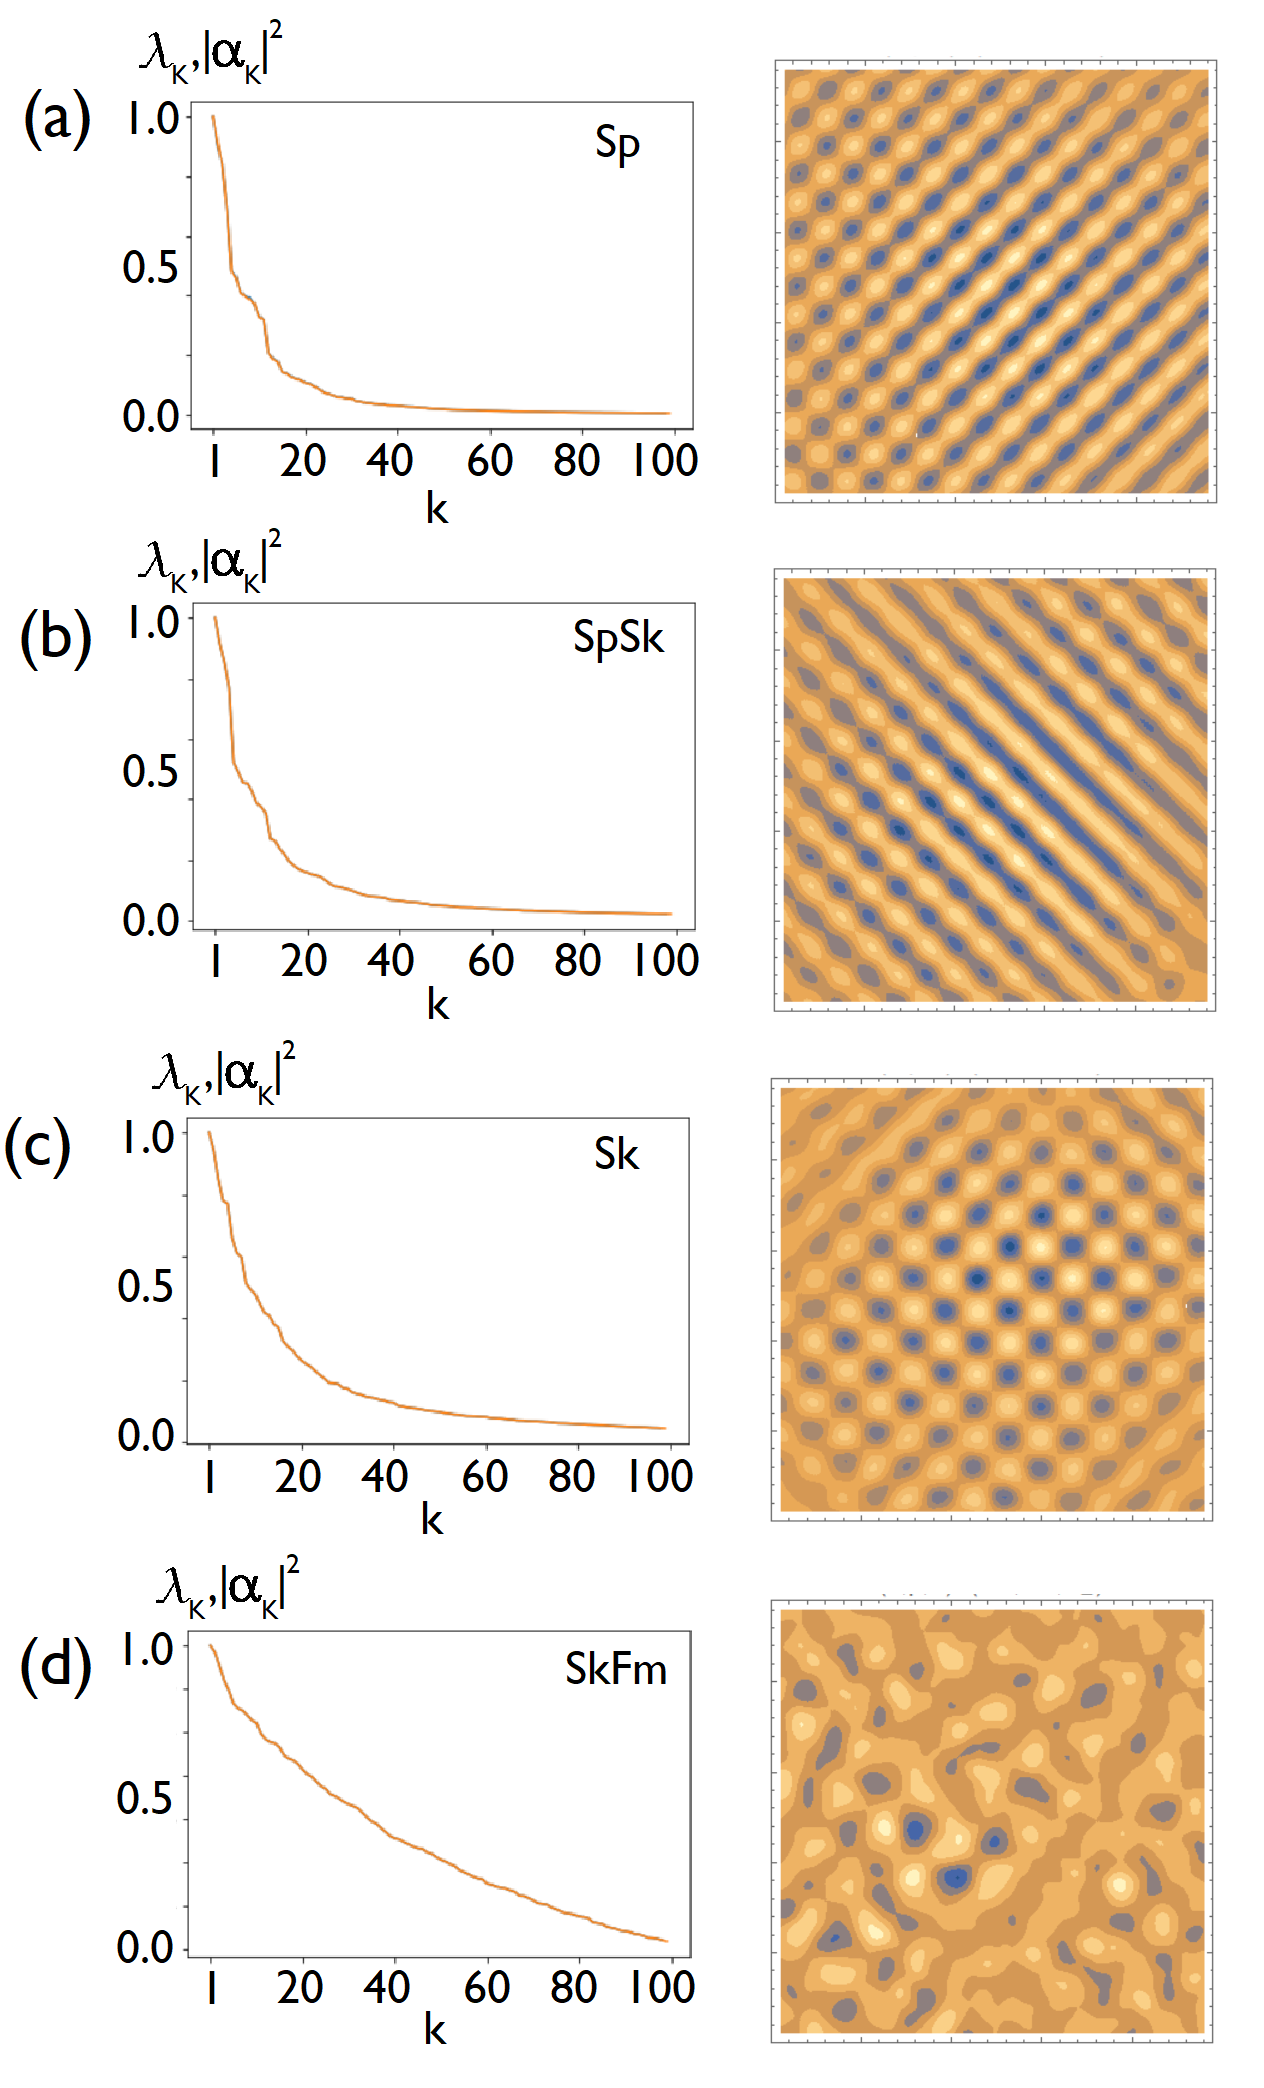
\includegraphics[scale=0.3]{fig1.png}
\caption{(left column) Leading eigenvalues $\lambda_k$ of the correlation matrix, normalized by the largest value $\lambda_1$. Completely overlapping results are obtained for average squares $\langle |\alpha_k |^2 \rangle / \langle |\alpha_1 |^2 \rangle$ [see Eq. (\ref{eq:alpha_k}) for definition] (right column) The first eigen-images ($k=1$) of the phases shown as plots of the $z$-component, $[{\bf I}_k ]_{iz}$. Rest of the leading eigen-images are shown in SM. ({\bf K should be k}) }\label{fig:0}
\end{figure}

\begin{figure}[h]
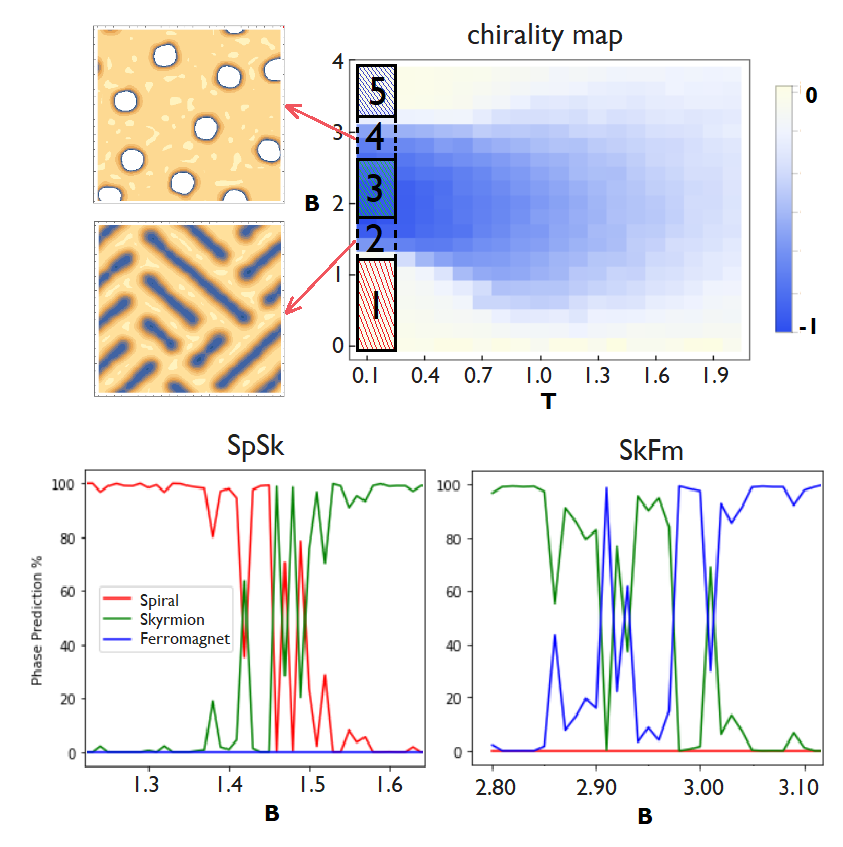
\includegraphics[scale=0.5]{fig2.png}
\caption{(top) Spin chirality [$\chi$ in Eq. (\ref{eq:m-and-chi})] in the $(T,B)$ plane obtained by MC calculation on the HDMZ Hamiltonian (\ref{eq:HDMZ}). Color scale represents the normalized value of the chirality. Boxes 1, 3, and 5 (2 and 4) represent regions where training (testing) data were taken for label predictions. Two configurations on the left show a typical SpSk and SkFm mixed state, respectively. The $z$-component of the local magnetization is used for the plots. (bottom) Probability of phase predictions in the SpSk and SkFm phases. The numbers represent averages over the testing set in the temperature interval $T\in[0.03,0.25]$ at the same $B$ value. The irregularities are not artifacts of the small data size.}\label{fig:1}
\end{figure}

Next, we follow the rapidly building tradition of applying ML classification scheme to the phase transition in condensed matter models and create a training set of configurations drawn from deep inside Sp, Sk, and Fm phases of the model (\ref{eq:HDMZ}) corresponding to 1, 3, 5 boxes in Fig. \ref{fig:1} respectively, and used the mixed phase SpSk (box 2) and SkSp (box 4) configurations as test sets. The aim was to see if the trained ML program could correctly capture the mixed nature of the phase. Details of the procedures used in the training and testing, and the ML architecture we used are all summarized in the Supplementary Material (SM). The results, shown as Fig. \ref{fig:1} (b) and (c), does not capture at all the smooth changes in the area fraction of the respective Sp and Sk (Sk and Fm) phases within the SpSk (SkFm) mixed phase.
It stands in stark contrast to earlier case studies on models exhibiting second-order phase transition. There, the ML program trained exclusively on the configurations deep inside the ordered and disordered phases could successfully predict the phases near the critical point in a continuously varying manner\cite{wang16,melko17,tanaka17,scalettar17,wetzel17,kim18,zhai17,scalettar17,beach18}. The ML program trained on the three distinct phases of the skyrmion model, on the other hand, fails quite dramatically to make continuously varying predictions for its mixed phases. Rather than declaring it as a failure, we view it as the way the neural network can successfully perceive the first-order phase transition - with a substantial mixed-phase region - differently from the sharp second-order transitions. At the same time, it is a telling suggestion that one must seek other means of characterizing mixed phases.

\begin{figure}[h]
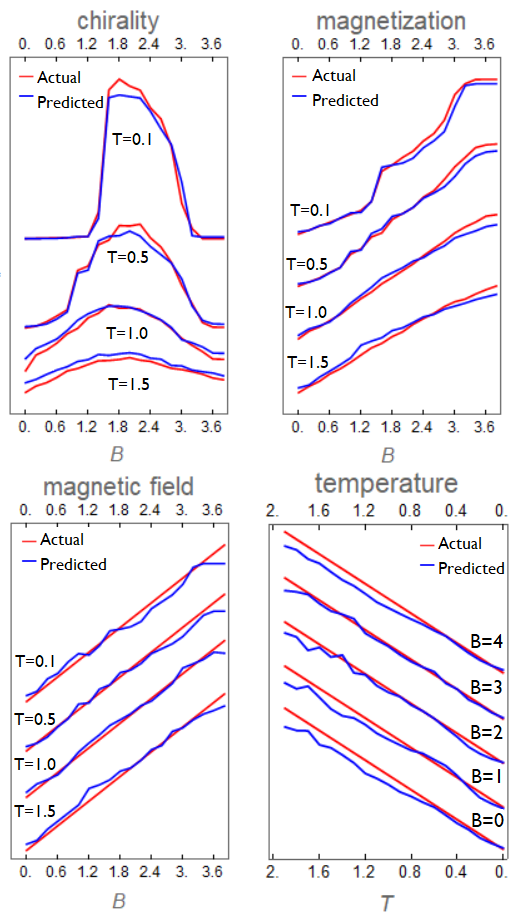
\includegraphics[scale=0.6]{fig3.png}
\caption{Machine-predicted values of $(\chi, m, B, T)$ in blue curves, compared to their actual values in red. The training and the testing were done on MC configurations generated by the Hamiltonian (\ref{eq:HDMZ}). Different curves are offset for clarity.}\label{fig:2}
\end{figure}

The main characteristics of the skyrmion and the ferromagnetic phases are the average spin chirality and the magnetization, respectively, defined as ($N$=number of lattice sites)

\ba
\chi & = & (1/N) \sum_i  ( \v n_i \cdot \v n_{i+\hat{x}} \times \v n_{i+\hat{y}} ) , \nn
%
m &=& (1/N) \sum_i n_i^z .  \label{eq:m-and-chi} \ea
%
The spiral phase is the one where none of these features takes on significant values. Instead of training the ML algorithm on the labels of configurations such as spiral, skyrmion, or ferromagnet, we train it on their features such as $\chi$ and $m$. Once the ML algorithm has been trained to predict those values correctly, the problem of labeling a given configuration is as good as solved. For instance an input configuration whose ($\chi$) $m$  is predicted to be near the the maximum allowed value can have no other label than skyrmion (ferromagnet). Intermediate values of both $\chi$ and $m$ signify the SkFm mixed phase. Finally, a configuration with small but non-negligible $\chi$ and $m$ are likely associated with the SpSk mixed phase. The labeling problem is delegated to the human decision, while the machine is left to do its work at predicting quantitative features of the input.

We carried out supervised learning of the $(\chi, m)$ features on configurations drawn from a wide temperature range $0.1 \le T \le 2.0$ ($\Delta T= 0.1$) and magnetic field $0 \le B \le 4.0$ ($\Delta B = 0.2$) corresponding to the entire chirality map in Fig. \ref{fig:1}. For each $(T,B)$ we collect 200 MC-annealed configurations for training purpose. The temperature and magnetic field intervals were sufficiently fine, as can be seen from the high quality of the pre-smearing data of $\chi$ in Fig. \ref{fig:1}. After training with a total of $200\times 20\times 21 = 82,000$ configuration, a fresh set of 40,000 configurations were generated to compare the machine-predicted $(\chi,m)$ against the actual values. As shown in Fig. \ref{fig:2}, the agreement between predicted and actual values is very good across the entire phase diagram.

Encouraged by the success of feature prediction in terms of $\chi$ and $m$, we next ask if the machine can be trained to recognize the particular temperature and magnetic field from which the input configuration originated. Figure \ref{fig:2} shows predicted values of $(T,B)$ to be very close to the actual values\cite{comment}. In contrast to $(\chi, m)$ which are the {\it mechanical variables} of the configuration, $(T,B)$ are {\it thermodynamic variables}. It turns out that ML
works well in predicting both kinds of features.
\\

\begin{figure}[h]
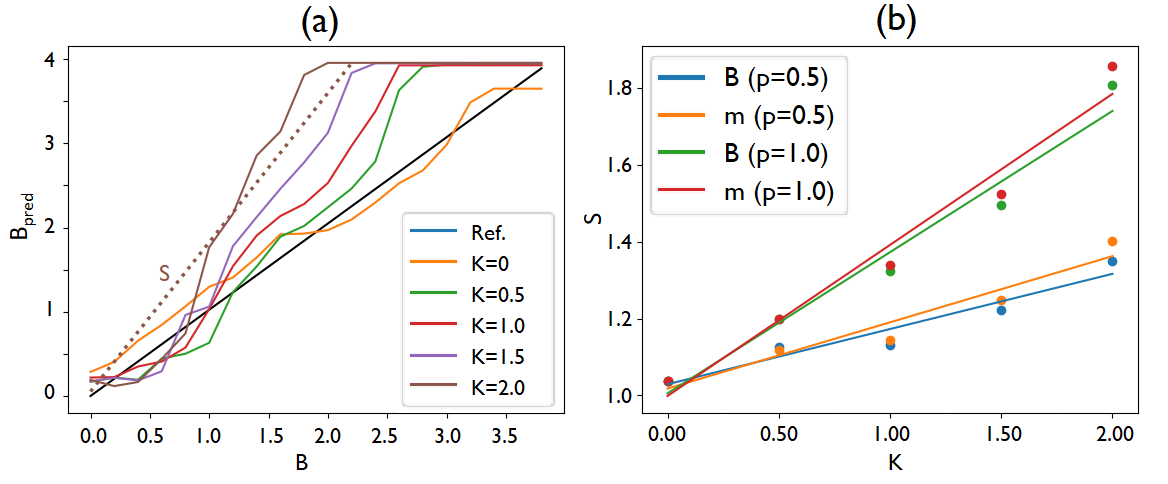
\includegraphics[scale=0.6]{fig4.png}
\caption{Machine prediction of $(\chi, m, B, T)$ for MC configurations drawn from $H_{\rm HDMZ} + H_K$ with $K=1$ and $p=0.5$.  The training itself was done on MC configurations generated by $H_{\rm HDMZ}$ alone.}\label{fig:3}
\end{figure}


Various modifications can be added to the HDMZ Hamiltonian (\ref{eq:HDMZ}) to represent the realistic situation of the material. One that reflects the disorder in the material can be given, for instance, by~\cite{skyrmion-book,jiang-review,fert-review}

\ba H_{K} = -K \sum_{i \in {\rm random}} (S^z_i )^2 . \ea
The magnetic anisotropy term of strength $K$ is added at the random sites occupying a fraction $p$ of the whole lattice. The model $H(K,p) = H_{\rm HDMZ} + H_K$ represents an adiabatically connected family of Hamiltonians as long as $K$ is sufficiently small compared to other energy scales. It is interesting to ask whether the ML algorithm, trained solely on  configurations drawn from $H(0,0)= H_{\rm HDMZ}$, can have predictive power over those generated from arbitrary $H(K,p)$. It is also a pragmatic question, when it comes to addressing the machine's predictive power over the experimental data, as real materials are never free of inhomogeneities and one does not have the {\it a priori} knowledge of the governing Hamiltonian.

%\begin{figure}[t]
%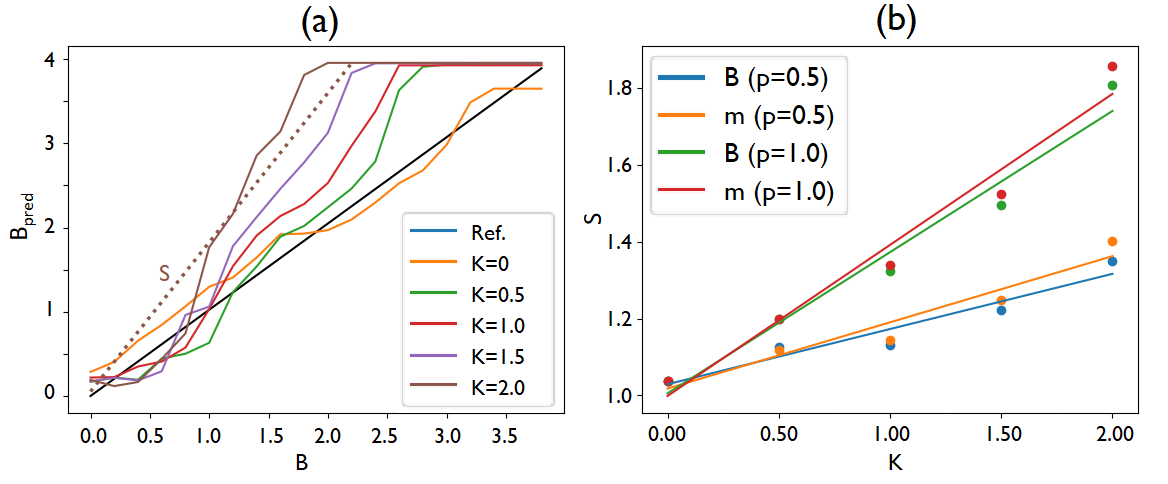
\includegraphics[scale=0.36]{fig4.png}
%\caption{(a) Predicted magnetic field $B_{\rm pred}$ at $T=0.1$, for several values of $K$ and $p=1$. The reference line in black is the actual $B$. A linear fit (dashed line) to the transient part of the curve gives the slope $s$. (b) The slope $s$ deduced from the $B_{\rm pred.}$ fit is shown as blue ($p=0.5$) and green ($p=1$) dots. They follow linear relationship as shown by lines of the same color. Twice the magnetic susceptibility $\alpha$ deduced from linear fits to $m_{\rm pred}$,  shown in yellow ($p=0.5$) and magenta ($p=1$), also gives the similar slope. Slopes for $p=1$ is larger than the slopes for $p=0.5$ in roughly obedience of the mean-field relationship $s = 2 K p \alpha$. } \label{fig:4}
%\end{figure}

\begin{table}[htb]
\begin{tabular}{ | ccc || ccc  cc  cc  cc |}
\hline
 & $(K, p)$ & & & $\Delta\chi$ &  & $\Delta m$ &  & $\Delta B$ & & $\Delta T$ & \\ \hline
 & $(0,0)$  &  & & 0.026 & & 0.027 & & 0.032 & &  0.028 & \\ \hline
 & $(1,0.5)$ & & & 0.030 & & 0.029 & & 0.060 & & 0.037 & \\ \hline
 & $(1,1)$   & & & 0.038 & & 0.024 & & 0.087 & & 0.066 & \\ \hline
 & $(2, 0.5)$ & & & 0.042 & & 0.025 & & 0.083 & & 0.064 & \\ \hline
 & $(2,1)$ & & & 0.042 & & 0.024 & & 0.152 & & 0.100 & \\ \hline
\end{tabular}\label{tab:PBC}
\caption{Averaged variance between predicted and actual values of $(\chi, m, B, T)$.}
\end{table}

A large number of configurations at $K=1.0$ and $p=0.5$ was generated by MC and tested by the ML algorithm, previously  trained solely on the pristine Hamiltonian $H_{\rm HDMZ}$. As shown as extensive data sets in SM, very good fits of all features $(\chi, m, B, T)$ were obtained. Similar plots for several $(K,p)$ values can be found in SM. The error in the prediction can be quantified by measuring $\Delta X \! \equiv \!  \sum_{i=T,B} \! | X_{\rm pred.} \! - \! X_{\rm act.} | / 400 $, where 400 refers to the total number of $(T,B)$ steps used in the generation of the test set, and $X=\chi, m, B, T$. Table I shows the mean errors in $(\chi, m, B, T)$ for several $(K,p)$ values. Both $\Delta \chi$ and $\Delta m$ remain less than 0.05 as $K$ grows from 0 to 2 (recall $J=1$ and $D=\sqrt{6}$). Note that $\chi$ and $m$ have the maximum size of 1. On the other hand, there is a systematic growth in $\Delta B$ and $\Delta T$ as $K$ becomes larger.

We plot predicted values $B_{\rm pred.}$ against the actual $B$ in Fig. \ref{fig:4}(a) for several $(K,p)$'s. There is an approximate linear relationship in $B_{\rm pred.}$ against $B$, at least until $B_{\rm pred.}$ reaches saturation, with the slope that grows almost linearly with $K$, as shown in Fig. \ref{fig:4}(b). The effect of the added anisotropy can be qualitatively understood within the mean-field picture by replacing $K  \sum_{i \in {\rm random}}  (n^z_i )^2$ with $2K p m \sum_{i \in L^2} n^z_i$, where $p$ is the impurity fraction. Assuming the magnetization $m$ depending linearly on $B$, $m = \alpha B$, the overall effect of the random anisotropy term is to replace the external field $B$ by the effective one, $B_{\rm eff} = (1+ 2K p\alpha ) B$. The machine, having been trained solely on pristine $H_{\rm HDMZ}$, knows nothing of the impurity effect {\it a priori} and ``erroneously" predicts the renormalized $B_{\rm eff}$ for the input, thereby incidentally divulging the discrepancy between the training and testing Hamiltonian.

Such expectations are consistent with our numerical analysis of Fig. \ref{fig:4}(b), showing almost linear increase in the slope of $B_{\rm pred.}$ with $K$. To further prove this picture we obtain $\alpha$ independently from linear fits to predicted $m$ values such as shown in Fig. \ref{fig:3}. The two ways of extracting the susceptibility $\alpha$ agree very well. The $\sim 2$ times difference in the estimated slopes for $p=0.5$ and $p=1$ data are consistent with the mean-field picture of $B_{\rm eff}$, as shown in Fig. \ref{fig:4}(b). The under-estimation of the temperature by the machine, as shown in Fig. \ref{fig:3} and SM figure 2, can be also understood, qualitatively, as a result of $K$ having the tendency to stiffen the spins and align them. At the same bare temperature $T$, configurations generated at finite $K$ tend to have more alignment of spins, which is ``erroneously" seen by the machine to be the consequence of lesser effective temperature $T_{\rm eff} < T$. Our numerical experiment demonstrates how well the neural network can respond to perturbations in the model~\cite{zhai18b}.

After extensive investigation of neural network training of skyrmion physics in the ML program, we pause to think about its implication for experimental data analysis. An increasing amount of information on skyrmion phase is being obtained by surface imaging techniques like LTEM and MFM. It has been customary to regard them as pictorial evidences of skyrmions but not much further analysis of the images have been done. Now combined with the PCA and neural-network training, we may be poised to feed these images through ML scheme to deduce physical features directly from the images, which include vital thermodynamic quantities such as magnetization, spin chirality, and correlation functions. As our experiment with the disordered Hamiltonian shows, the ML program can see beyond the simplest model Hamiltonian and extract relevant features correctly from experiments where the governing Hamiltonian is undoubtedly more complicated. It can be used as an interesting ``recovery tool" predicting the magnetic field and temperature whence the data was obtained. Further close interplay between imaging scientists and ML scientists can create a new research potential for the skyrmion science and other image-driven surface science such as the scanning tunneling microscopy.

This work was supported by Samsung Science and Technology Foundation under Project Number SSTF-BA1701-07.

\begin{thebibliography}{99}

\bibitem{melko16} G. Torlai and R. G. Melko, Phys. Rev. B {\bf 94}, 165134 (2016).

\bibitem{wang16} L. Wang, Phys. Rev. B {\bf 94}, 195105 (2016).

\bibitem{melko17} J. Carrasquilla and R. G. Melko, Nat. Phys. {\bf 13}, 431 (2017).

\bibitem{melko17b} P. Ponte and R. G. Melko, Phys. Rev. B {\bf 96}, 205146 (2017).

\bibitem{melko17c} A. Morningstar and R. G. Melko, arXiv:1708.04622 (2017).

\bibitem{tanaka17} A. Tanaka and A. Tomiya, J. Phys. Soc. Jpn. {\bf 86}, 063001 (2017).

\bibitem{scalettar17} W. Hu, R. R. P. Singh, and R. T. Scalettar, Phys. Rev. E {\bf 95}, 062122 (2017).

\bibitem{wetzel17} S. J. Wetzel and M. Scherzer, Phys. Rev. B {\bf 96}, 184410 (2017).

\bibitem{wetzel17b} S. J. Wetzel, Phys. Rev. E {\bf 96}, 022140 (2017).

\bibitem{iso18} S. Iso, S. Shiba, and S. Yokoo, Phys. Rev. E {\bf 97}, 053304 (2018).

\bibitem{kim18} D. Kim and D.-H. Kim, arXiv:1804.02171v1 (2018).

\bibitem{zhai17} C. Wang and H. Zhai, Phys. Rev. B {\bf 96}, 144432 (2017).

\bibitem{beach18} M. J. S. Beach, A. Golubeva, and R. G. Melko, Phys. Rev. B {\bf 97}, 045207 (2018).

\bibitem{zhai18} C. Wang and H. Zhai, arXiv:1803.01205 (2018).

\bibitem{russian18} I. A. Iakovlev, O. M. Sotnikov, and V. V. Mazurenko, arXiv:1883.06682v1 (2018).

\bibitem{nagaosa-review} N. Nagaosa and Y. Tokura, Nature Nanotech. {\bf 8}, 899 (2013).

\bibitem{skyrmion-book} J. P. Liu, Z. Zhang, and G. Zhao, {\it Skyrmions: topological structures, properties, and applications} (CRC Press, 2016)

\bibitem{jiang-review} W. Jiang, G. Chen, K. Liu, J. Zang, S. G. E. Velthuis, and A. Hoffmann, {\it Phys. Rep.}
{\bf 704},1 (2017).

\bibitem{fert-review} A. Fert, N. Reyren, and V. Cros, Nature Reviews Materials {\bf 2}, 17031 (2017).

\bibitem{han-book} J. H. Han, {\it Skyrmions in Condensed Matter}  (Springer, 2017).

\bibitem{tokura10} X. Z. Yu, Y. Onose, N. Kanazawa, J. H. Park, J. H. Han, Y. Matsui, N. Nagaosa, and Y. Tokura, Nature (London) {\bf 465}, 901 (2010).

\bibitem{goodfellow} I. Goodfellow, Y. Bengio, and A. Courville, {\it Deep Learning} (The MIT Press, 2016).

\bibitem{comment} Averaging is done over the MC configurations generated at a fixed $(T,B)$. Shown in the figures 2 and 3 are the averages of the machine-predicted values, and the averages of the actual values. There is a greater degree of fluctuation if the predictions of an individual configuration is compared with the actual value of that configuration.

\bibitem{SM} Supplementary Material

\bibitem{zhai18b} Y. Wu, P. Zhang, H. Shen, and H. Zhai, arXiv:1802.03930 (2018).

\end{thebibliography}

%\bibliographystyle{apsrev}
%\bibliography{reference}


\end{document}
